In the following we will outline the design of \thename{} and give a detailed
description of each area of functionality. The design is heavily tied to the
\thename{} specification, but further includes some considerations for
implementation, i.e.~the design of the implementation.

As previously mentioned, the primary aim of \thename{} is to provide an abstract
machine that is capable of supporting most of the modern programming paradigms
in an efficient manner. The overarching idea is that by exposing much of the
underlying low-level constructs we provide very flexible means for compilers to
do things the way that is most suitable for their particular requirements,
without having to conform to a tight object-model or strict type system. This
involves exposing constructs like scopes, object model internals, thread
management and the type system. Further the type system is aimed at being strict
enough to guarantee type safety as far as possible, but flexible enough for
dynamic languages. Compilers are free to select which features to utilize,
meaning for instance that for a strictly statically typed language, the dynamic
typing mechanisms can be disregarded and all method dispatches can be wired
statically.

\textbf{Note:} Because the specification is such a central document to the
design we will not cite it directly throughout the thesis. Instead we refer to
Appendix~\ref{sec:appendix:spec} where it is included in its entirety.

\subsection{Memory and Object Model}

\thename{} uses the common stack and heap memory model. Each running thread has
its own evaluation stack that is local to itself. Other threads, whether parent
or child can not access elements on another thread's stack, neither by direct
memory addressing or by use of the \code{StackReference} type. The only means by
which a thread can make data from its stack available to others is by boxing it,
i.e.~moving it to the heap and track it by a reference. The heap is a single
globally shared memory region where data is stored and modified by use of
references. It is managed fully by the garbage collector, which means that all
allocations and deallocations are made through a single interface. Internally
the garbage collector is regarded as a ``black box'', meaning that no
assumptions to its inner workings are made, and it is assumed to efficiently
free unused memory when possible. The only exception to this is that the object
model defines a sub-routine on heap objects called \code{finalize} which is
called before the garbage collector releases the object's memory. It is used for
an object to be able to properly free any resources it might be using, such as
open files or network connections, and is directly analogous to C++'s destructor
method on classes.

The object model defines how objects are laid out in the heap, how their content
is described by the type system and how it is referenced from the
stack. \thename{} uses a simple but very flexible object model. The general idea
is that a heap object is described by the \code{Composite} type which is capable
of expressing arbitrarily complex data structures. In addition to what is
described by the type, a heap object includes a reference to an object of the
\code{AnyType} type. The purpose of this is to provide language implementations
the means to associate some arbitrary information to objects. It could used for
any kind of metadata storage, implementation of class methods, polymorphism,
etc.

\subsection{Execution Model}
\label{sec:design:exec}

The model of execution defines how, where and by whom code is executed during
run-time. All code in \thename{} is executed in the context of a thread (details
in Section~\ref{sec:design:threading}), and all threads are spawned from the
initial ``main'' thread in which execution begins. This allows language
implementations to use the multi-threading features of \thename{}, but also to
ignore them and run everything in a single thread without having to worry about
creating and destroying threads.

\subsubsection{Sub-routines and Calling Convention}
\label{sec:design:exec:sub-routine}

A sub-routine is a set of instructions that can be executed, or invoked, as a
group from another instruction, in our case the \instr{invoke} family of
instructions. \thename{} does not currently support either static or dynamic
linking and hence all byte code is stored in a single stream of bytes. A
sub-routine is simply defined by a designated subset of those bytes that,
usually, performs a specific task and subsequently passes control back to the
caller. In \thename{} each sub-routine has a name, a low-address that is the
entry point, and a high-address which is the last instruction byte belonging to
it. The machine does not restrict the address bounds, so the same code bytes can
potentially be shared by multiple sub-routines, however rare that scenario might
be. In addition they define the type of arguments that are expected to be found
on the stack.

Most CPU architectures define a \textit{calling convention} which defines how
parameters are passed to sub-routines and how values are returned from
them. Parameters to a sub-routine must be pushed into the stack prior to an
\instr{invoke} instruction. The sub-routine code can then peek upward into the
stack to retrieve or replace them. \thename{} has no notion of return values as
commonly used by other architectures. Instead the callee allocates space on the
stack and sub-routines must accept corresponding parameters which it can then
``fill'' with the values that are to be returned. This is a flexible method that
allows any number of values to be passed back to the caller, and further does
not require any dedicated instructions for returning values.

\subsection{Scopes}
\label{sec:design:scopes}

At its core, a scope is simply a mapping from names to values that define the
bindings available at any given point during execution. The available bindings
depend on the scoping rules used, and can generally be divided into the two
mechanisms: dynamic and lexical. With dynamic scoping a name is resolved when it
is \emph{evaluated}, that is, it depends on the execution context or state of
the program. With lexical scoping a name is resolved when it is \emph{defined},
meaning that resolution depends on the name's lexical location in the source
code. Dynamic scoping can be confusing and make it difficult to reason about a
program's behavior. It can lead to unwanted or unexpected results because the
programmer has to be very careful not to use identical names in different
locations that might be evaluated in the same execution context. Lexical scoping
makes it easier to figure out what a program will do and harder to shoot
yourself in the foot. While dynamic scoping has more or less disappeared from
modern language implementation\cite{cse341} it is still used in some places. An
interesting example are C macros (and indeed macros in general) which do no form
of resolution by themselves, it is essentially simple text replacement. Macros
are a prime example of how dynamic scoping can be very useful, but also of the
severe issues and frustration that it can cause.

Scopes are usually organized in tree structures, where each scope has exactly
one parent and zero or more children. Name resolution starts in one specific
scope, and if a matching name is found then the value of the name is determined
immediately. If the name is not found in the current scope then resolution
continues in the scope's parent, repeatedly. As a result, a name can be
overridden, known as \textit{shadowing}, by a child scope by binding a value to
a name that is also used by the parent scope.

\thename{} exposes run-time functions for managing scopes, more specifically
pushing and popping them on demand. That means that by default a new scope is
\emph{not} introduced when a sub-routine is invoked, compilers must handle this
manually. This way a compiler is completely free to introduce scopes according
to the semantics of a language specification, and there is very little
performance overhead by manual scope management; the internal procedures are the
same as if the machine would introduce scopes automatically.

Scopes can be used to as the means to implement various different language
features. A global scope like C's or JavaScript's can be achieved simply by
having all other scopes be children (or grand-children) of it. Module systems
like Java's \code{package} and \code{import}, can be constructed by combining
multiple scopes into a larger context specific for each module. On a more
detailed level, C-like languages introduce new scopes in every block, usually
marked with braces, such as if-statements, switch cases, function bodies and so
on.

\subsection{Executable File Format}

\thename{} reads executable files written in the Executable Linkable Format
(ELF). ELF is a widely used format for executable binary files that is standard
on Unix based systems\cite{wiki-elf}. It is a simple and very flexible format
that is not specific to any platform or architecture but is a container format
for such. That means that it provides structures for organizing bits and bytes
into sections and defining headers that describe the file in terms of purpose
and functionality.

ELF files are not necessarily executable files, they can be only linkable (hence
the name) meaning for instance, that there is no execution entry point
defined. \thename{} does not currently support linking, which is why we will not
go into details about linkable files; this section is about executables only,
but most of the information applies to both.

The contents of an ELF file is stored in segments which in turn contain
sections. Generally speaking, segments contain information that is useful for
the execution of programs while sections are useful for linking. The data
contained in both is the same, but the distinction provides different views of
that same data, useful for said purposes\cite{elf-spec}. However, since the
format by design is flexible and can be used in whatever manner and for whatever
purpose desired. There are no restrictions by the format per s\'e.

An ELF file is described by headers defined in the file itself. The overarching
file header that describes the remaining file organization is the `ELF
header`. It details the attributes of the file such as the architecture on which
the file can be executed, endianness, ELF format version and so on. Further it
defines where in the file that section and segment headers are located, their
size and how many there are. In turn the section and segment headers describe
their entries in the same manner. The general idea is that the starting
location, size of entry and amount of entries is defined and from that the data
can be extracted correctly.

The fact that ELF is such a widely used format, and standard for Unix systems,
enables much easier porting of existing tools and libraries to run on
\thename{}. GCC and GNU Binutils\footnote{GNU Binutils:
  \url{http://www.gnu.org/software/binutils}} are examples of software that is
portable, and indeed is designed to be relatively easy to port to new
architectures. That effectively means that an extensive compiler collection and
tools are available at a fraction of the effort that it would take to implement
them from scratch.

\subsection{Information Tables}

\thename{} executable files define three distinct kinds of information tables
which are used to store most information that is referenced by the byte
code. The exceptions are inlined literal values and jump tables for the
\instr{switch} instruction (explained in
Section~\ref{sec:design:isa:control-flow}). Byte code makes references to
entries in the tables by use of indices produced by compilers, and which are
given by integral values. Indices are private to each table so an index value
will point to different entries depending on which table a given instruction
assumes that the index is into.

The most simple table is the string table which is a list of immutable UTF-8
character strings. It is used to store and retrieve any string that a program
might use, both for identifying scope symbols, run-time functions, fields
etc. It is also the place where compilers must store strings that are used in
ordinary program logic. All strings found in the string table must be unique,
both because it is redundant to store duplicates and because it enables the
machine to compare strings for equality simply by comparing their indices. That
saves a lot of look up operations which would otherwise sum up to a significant
performance cost.

Rather than using the regular UTF-8 encoding standard, we have chosen a
derivative version named Modified UTF-8. This encoding has the UTF-8 character
{\tt U+0000} encoded as the bytes {\tt 0xC0}, {\tt 0x80}, rather than a null
byte ({\tt 0x00}). This enables functions to interpret UTF-8 strings as regular
null-terminating strings, which is how the C Programming Language handles
them.

Next is the constant table that contains any type of value for use in
programs. Values are retrieved by a program by use of the \instr{pushConstant}
instruction which takes an index into the table and pushes the value onto the
stack. It is useful for handling large data types that can be expressed neither
in the default \code{Int8} argument type nor the large \code{Int32} enabled by
the \code{large} prefix. Constant entries can be arbitrarily large and can thus
also be used to store array literals. In some cases a compiler will be able to
optimize the total code size by storing recurring constant values in the
constant table rather than inlining them in instructions.

The last and most complex table is the meta-data table. It contains information
about all types, sub-routines and fields. All entries are represented in the
DWARF debugging format (explained in Section~\ref{sec:design:types:dwarf}) which
is parsed by the machine into internal data structures. Meta-data is retrieved
similar to constants, by use of the \instr{pushMeta} instruction.

These three tables together are similar to JVMs concept of a constant pool that
``[...] contains several kinds of constants, ranging from numeric literals known
at compile-time to method and field references that must be resolved at
run-time.''\cite[Section 2.5.5]{jvm-spec}.

\subsection{Stack Management}
\label{sec:design:stack-mgmt}

A stack is an abstract data structure, fundamental for many fields of computer
science. At its core it is a simple model consisting of two essential functions,
{\it push} and {\it pop}, as visualized in Figure~\ref{fig:stack}. Push adds an
element to the top of a stack, while pop removes the top-most element. As an
analogy, imagine a pile of dishes: when adding a new dish it becomes the new
top-most dish in the pile, and you can only remove the most recently added
dish. This sequence of adding and removing from a collection of elements is
called Last In, First Out (LIFO).
\begin{figure}[h]
  \centering
  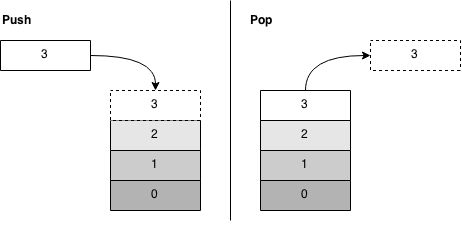
\includegraphics[scale=0.6]{images/stack.png}
  \caption{Stack push and pop operations}
\label{fig:stack}
\end{figure}

Although one cannot pop the second element from the top without first removing
the top most element, the model can easily be modified to support such
operations. For instance, a common stack operation is that of reading the value
of an element a number of slots into the stack without modifying anything, known
as {\it peeking}.

The most common notation in arithmetic formulas and statements are the infix
notation, where the operator is written between its operands: $1 + 2$. One can
express the same statement with prefix notation, also called \term{Polish
  notation}: $+\ 1\ 2$, a style commonly used in the family of Lisp
languages. When programming stack machines, one uses what is called the
\term{reverse Polish notation}, which is in fact postfix notation: $1\ 2\ +$. By
using this notation, one can easily convert this into stack operations, where
$1\ 2\ +$ becomes:
\begin{stackops}
  \op{push 1}{1}
  \op{push 2}{2,\ 1}
  \op{add}{3}
\end{stackops}

Here the {\tt add} operation pops two elements, adds them together and pushes
the result back onto the stack.

\subsubsection{Stack Organization}

Stacks in \thename{} are unbounded, meaning that they can be arbitrarily large
and that stack overflows can never occur (if the machine runs out of memory
entirely it is treated as a memory error, not a stack overflow). Throughout the
report, we will say that the stacks \term{grows downwards}. This is because
physically, the top most element of the stack is located at the highest address
in memory. Therefore, as more elements are pushed onto the stack, they will get
higher addresses, making the stack grow downwards in memory.

A stack element consists of some type information along with the actual data
bytes. The type information consists of a declared type and an actual type. For
statically typed languages, these will most likely be the same. For dynamic
languages this is useful for keeping track of an element's type, as it, in some
cases, is allowed to assign a value to an element which is different from the
originally declared type. This only concerns abstract data types, which we will
get back to in Section~\ref{sec:design:types}, when discussing the type system.

\subsubsection{Stack Manipulation}

As mentioned above, there are instructions for doing simple stack manipulations
such as \instr{push} and \instr{pop}. As we will see later, these two instructions
alone are very limiting, and make the job of writing a compiler very
tedious. Therefore we will need more expressive instructions that simplifies
complex stack manipulations.

When we later describe the execution model of the machine, we will see that we
need instructions for storing and retrieving elements further up the stack. For
instance, if we want to access the arguments given to a sub-routine, they will
be located upward in the stack. The compiler will need an effective method of
duplicating those elements onto the top of the stack, making it accessible for
further computation. Also it will need to store an element back to a specific
position up the stack, i.e.~replacing an element, effectively returning a value
to the caller.

Such versions of the push and pop operations will take a displacement argument,
defining how many places up the stack it is to push to or pop from. To make this
as convenient as possible, the displacement will be from the top of the stack,
meaning displacement 0 will be the top of the stack, 1 is the second to the top
element and so on.

To address this, we have the instructions \instr{pushElement} and
\instr{storeElement}. The former will take the element at the given
displacement, without removing it, and push it onto the top of the stack. The
latter will pop off the top-most element and push it to the given displacement,
effectively overwriting that element. This convention requires that the caller
has pushed an element onto the stack with the sole purpose of being
overwritten.

There are separate instructions for adding new elements onto the stack, namely
\instr{pushLiteral} and \instr{pushConstant}, which are \thename{}'s version of
the simple \instr{push} instruction.

Here we can see some simple operations using the \instr{pushElement} and
\instr{storeElement} instructions.
\begin{stackops}
  \op{-}{3,\ 1,\ 1}
  \op{pushElement 0}{3,\ 1,\ 1,\ 3}
  \op{storeElement 2}{3,\ 3,\ 1}
\end{stackops}

\subsection{Threading}
\label{sec:design:threading}

Big chip manufacturers like Intel, have always been under big pressure to
deliver ever faster processors, year after year. For around the last decade, the
technological development of processors has been focused on adding cores rather
than increasing the clock speed, which already started to stagnate around
2004\cite{sutter}. With multiple cores per processing unit, popularly called a
multi-core processor, processes may actually run in parallel, i.e.~running at
the same time, rather than just concurrently where multiple processes actually
share the same processor.

A thread is typically the smallest sequence of executable instructions handled
by a processor. A process being run by an operating system therefore has one
thread which the operating system's scheduler delegates CPU-time to, allowing it
to execute said instructions. With multi-core processors, the notion of a single
process having multiple threads arose, making it possible for tasks to run
concurrently. A process utilizing this feature is called multi-threaded.

Although multi-threading is a very interesting feature, it also raises a lot of
challenges when designing the execution model. Different threads cannot directly
read and write to the same location, or address, in memory without taking data
races into account, which is a common mistake when writing multi-threaded
programs. If multiple threads are reading and writing to the same memory, it is
impossible for the threads to base any logic on it, as another thread can change
its value at any time, effectively pulling the rug out from under you. This
problem as been named the \term{mutual exclusion problem}, and is solved by
using synchronization structures, such as semaphores and monitors.

\thename{} supports threading and synchronization structures therefor. As we are
using a stack machine, each thread has to have its own state, including its own
stack. In other words, all stacks are private and cannot be shared across
threads. This can however be facilitated by using heap object which are
referenced from multiple threads' stack.

\subsubsection{Thread Pool}

Creating and destroying system threads is not free. If a new thread is created
on demand it would create significant overhead. Another problem with this model
is the risk of resource thrashing. If there is no limit to the number of threads
that can be created, it can intentionally or unintentionally be exposed to heavy
abuse. A solution to both of these challenges is having what is called a
\term{thread pool}. Upon machine initialization, a fixed number of threads is
pre-initialized and stored in a data structure. When a thread tries to spawn a
new thread, it is given one from the thread pool, and if the thread pool is
empty, it has to wait for a thread to become vacant.

This model, although effective, also brings with it some
challenges. Specifically, when the thread pool is empty, the spawning thread
cannot stop and wait (busy-waiting) until a new thread is vacant, as this would
block the whole thread. Rather, the machine will use a work queue, which manages
the thread pool so other threads does not need to wait for a thread to become
vacant, and afterwards fight with each other about whom gets to take it. The
spawning threads would give the task which it wants run in a new thread, to the
work queue. The queue would monitor the thread pool and as soon as a thread
becomes free, it would take the task first in the work queue and run in. This is
called scheduling and constitutes a whole field of research per s\'e.

\subsubsection{Errors and Exceptions}

Two types of errors can occur; internal errors in the machine and errors
produced by the program that the machine is executing. Internal errors will most
likely occur in some child thread and not in the process' original thread. If
that is the case we can stop that thread and gracefully stop the machine if it
cannot safely continue. If the error occurs in the process' original thread, we
will in most cases still be able to catch the signal sent by the operating
system and exit gracefully.

When the program being executed produces an \term{exception} it will percolate
up through a defined set of user-defined exception handlers until it is
handled. If there is no way of handling the exception it is called an uncaught
exception, and the machine will print some information on the exception and
stop. It will not attempt to join all threads as it cannot know how long this
would take. Therefore all threads are exited and memory is freed, ensuring no
memory leaks.

\subsection{Types}
\label{sec:design:types}

The type system of \thename{} aims to enable efficient implementation of both
dynamically and statically typed languages. That gives rise to a need for an
adaptable system that is capable of expressing arbitrarily complex types along
with potential storage layout information for languages that require explicit
memory layout of objects. Moreover the system must be flexible and modifiable
during run-time, e.g.~to allow dynamic languages to add and remove members of an
object while still being able to properly type check the code.

\subsubsection{DWARF}
\label{sec:design:types:dwarf}

Types are expressed in the DWARF format\cite{dwarf} which is a format mainly
used to describe debug information for executable files, essentially by
describing the source code of a program and mappings into to the compiled
binary. It is used in many modern compilers\footnote{Usages include GCC, Clang
  and Go} and is commonly used in combination with ELF binaries. It provides a
way to describe everything from source code locations, scopes and exception
handling to compilation units, linking information and shared libraries. The
primary building block of DWARF information is the Debug Information Entry
(DIE). It consists of a DWARF tag that describes the kind of entry, and a set of
attributes that further defines the characteristics of an entry. Tags and
attributes can be nested which enables types to be as intricate as necessary. It
is worth mentioning that DWARF is simply a \emph{format} specification, and
while there are libraries to help read and write the format, they are not part
of the DWARF specification.

We do not use the full set of features provided by DWARF, rather we only use
DIEs for type information in ELF files. We would most likely also use DWARF to
facilitate proper debugging, but that is beyond the scope of this project.

DWARF DIEs are tree structures for which we will use indention based notation to
present. Listing~\ref{lst:design:dwarf:basic} shows how we can use DWARF to
express a 32-bit signed integer. Note that the name ``int'' has no special
meaning in DWARF, but consumers of DWARF may put special meaning into names.

\begin{lstlisting}[
  caption={A simple DWARF DIE describing a 32-bit signed integer},
  label={lst:design:dwarf:basic}]
<1> DW_TAG_base_type
        DW_AT_name = int
        DW_AT_byte_size = 4
        DW_AT_encoding = signed
\end{lstlisting}

In the above, there is a single tag with three attributes that describe the
type's name, size and encoding. The \code{DW\_TAG\_base\_type} essentially
designates a primitive type, one that is not a compound of one or more types,
and will usually be a leaf in the DWARF tree. For types that \emph{are}
compound, the approach is to store DIEs in an indexed table and reference types
by their index location in the table. In the above, the type's index is
designated by the \code{<1>}. By doing this no type ever has to be duplicated,
because any other type can simply reference it by its index. Tags start with the
\code{DW\_TAG\_} prefix while attributes use \code{DW\_AT\_}, all of which are
simply names for integer constants defined by the DWARF specification.

Listing~\ref{lst:design:dwarf:complex} shows a more complex example with a
subprogram (i.e.~a sub-routine) that returns a pointer to the integer type
defined above.

\begin{lstlisting}[
  caption={A more complex example of DWARF types referencing each other},
  label={lst:design:dwarf:complex}]
<2> DW_TAG_pointer_type
        DW_AT_byte_size = 4
        DW_AT_type = <1>

<3> DW_TAG_subprogram
        DW_AT_name = foo
        DW_AT_type = <2>
        DW_AT_low_pc = 0x1
        DW_AT_high_pc = 0x10
\end{lstlisting}

It is shown how type \code{<2>} is defined as a pointer to the type \code{<1>},
which in C lingo would be \code{int*}. Type \code{<3>} defines a sub-routine
whose name is ``foo'' and returns a \code{<2>}, again in C lingo that would be
\code{int (*foo)(void)}. This is the fundamental way that the DWARF format
expresses types; it is simple, yet very flexible and powerful.

There are scores of attributes and tags defined in the specification, but we do
not nearly use all of them. Because the format is so simple it is easy to add
new tags and attributes by defining a name for the new entry and a corresponding
numeric constant and documenting it.

DWARF DIEs are, as mentioned, tree structures which is effective for expressing
types but is not very compact for storage, and can result in potentially
unwieldy type data. There are more than one way to store the tree structure in a
compact manner, one of which we will describe here. %XXX fjern eller skriv om
                                                    %LEB128

\subsubsection{\thename{}'s Types System}
\label{sec:design:type-system}

\thename{} provides a set of built-in types, encompassing both primitive types
as well as references, arrays and composite types. Further there is the concept
of a meta kinds which essentially wraps type definitions, type references,
sub-routines, etc.~into a unified metadata kind which are all stored in a single
table in the executable.

Compilers can map their primitive types to the ones provided by \thename{}, and
we expect that combinations of the available compound types to be sufficient for
expressing any other conceivable type however complex.

Below is a description of the various kinds of simple types provided.

\begin{description}
\item[Integers] \hfill\\
  Integer types include all combinations of 8-, 16-, 32- and 64-bit, signed or
  unsigned, integer numbers. E.g. {\tt Int32} and {\tt UInt16}.

\item[Boolean] \hfill\\
  A Boolean type with the possible values of `true` or `false`.

\item[Floating-point numbers] \hfill\\
  Non-integer numbers will be represented by floating-point precision numbers,
  either 32-bit or 64-bit, named {\tt Ieee32} and {\tt Ieee64}. These will
  respectively follow the IEEE~753-1985 and IEEE~754-1985 standard of
  representation.

\item[Address] \hfill\\
  Unsigned integer value representing a memory address, named {\tt Address}.

\item[Abstract types] \hfill\\
  A type which can take any value at run-time, named {\tt AnyType}. Large stack
  initialized values will be boxed on the heap to make space for them.
\end{description}

The IEEE-753 and IEEE-754 standards does not specify an endianness for storing
or transferring floating-points numbers, hence we will conform to the school of
big-endian, as done through the entirety of \thename{}.

% reference

The machine has a set of reference types, with the most fundamental being the
{\tt Reference <t>} type. This allows heap objects to be referenced from the
stack. It is an example of a compound type that defines the type of the object
it references by referring to another type definition. In the opposite scenario,
there is a {\tt StackReference <t>} type, allowing passing of references
directly to stack references.

To support variable argument calling conventions, i.e.~letting a sub-routine
take an arbitrary number of arguments, a special reference type is needed. This
is done through an {\tt ArgumentReference}, allowing a sub-routine to iterate
over its given arguments.

% arrays

\thename{} supports two types of arrays; a static fixed length and a dynamically
sized kind. Both are compound types that define the type of its elements. This
could be to other arrays, allowing an array to be multi-dimensional without
specialized types. The static variant additionally defines a lower and upper
index of available slots. The dynamic variant does not define those limits as it
can grow dynamically during run-time, because of which it will be always be
located on the heap. It will therefore be referenced through a {\tt Reference}
type.

% composite

To support compound types similar to a struct in C, there is a {\tt Composite
  <t+>} type. This is a collection of an arbitrary number of other types,
describing its member. Though not visible from the type signature, each member
has a name, allowing for convenient referencing.

% meta

% TODO: review
Lastly, the machine has a set of meta types, describing various kinds of data in
the machine, including types them selves. This is required for allowing programs
to operate on types and to support concepts such as reflection. There will be a
specific type of instructions designed for utilizing this feature, which will be
explained further in the following section.

Below we see a brief description for each meta type supported:

\begin{description}
\item[Type:] A kind of meta information describing one of the above types.

% \item[Metadata:] \ \\ %TODO include?

\item[Field definition:] Describing a heap object field, with name, type of
  value and possible properties.

\item[Sub-routine definition:] Describing a sub-routine with name, types of the
  parameters, and address of its containing instructions.

\item[Sub-routine reference:] Reference to a sub-routine by name.

\end{description}

\subsection{Instruction Set Architecture}
\label{sec:design:isa}

The interface by which compilers and programmers interact with \thename{} is
defined by the Instruction Set Architecture (ISA). It is the language that the
machine understands and provides the means to utilize all of available
functionality. It is exactly the same as the x86 instruction set is to the x86
CPU architecture.

The \thename{} ISA is a set of instructions which are relatively high-level, as
compared to ordinary hardware implemented instruction sets. The abstraction
level of the \thename{} is aimed at being high enough for straightforward
implementation of high-level constructs but low enough for efficient code
generation and execution. It can be divided into four overarching categories of
functionality, namely stack manipulation, numeric operations, control flow and
heap related instructions.

Most instructions require one or more parameters that define the exact behavior
of execution. By default, the arguments are read from the byte code stream, but
several instructions have \emph{indirect} variants that read one or more of
their arguments from elements on the stack instead of from the byte code
stream. This enables much more flexible and dynamic programs because arguments
to an instructions can be computed at run-time rather than having to be
statically determined.

There is a set of instruction \emph{prefixes} that modify how an instruction is
interpreted in terms of arguments, safety and exception handling. Technically
they are simply predefined byte values that are parsed before an instruction is
executed. For instance, integer arguments are by default read as 8-bit values,
but may be extended to 32-bits by providing the \code{large} prefix. Another
prefix, \code{noOverflow}, will make overflowing arithmetic throw an
exception. Prefixes only take effect for a single instruction and are reset at
the end of every instruction cycle.

The following describes each of the four categories of instructions in detail
and highlights some of the most interesting examples.

\subsection{Stack Manipulation}

The stack manipulating instructions facilitate the functionality described in
Section~\ref{sec:design:stack-mgmt}. It can be argued that all instructions are
stack manipulations since almost every instruction will leave the stack
changed. However we define stack manipulations as the instructions that either
add or remove an element on the stack without causing \textit{side effects},
which is essentially anything that results in changes in the heap. Neither
control flow nor numeric instructions are considered stack manipulations.

The stack manipulating instructions mostly consist of set of push-instructions
that push values onto the stack. What that values represent and how it is
obtained differs between the individual instructions, the most fundamental of
which are described below.

\begin{description}

\item[\instr{pushElement}:]

  Fetches an element from upward into the stack and pushes a copy back onto the
  stack. This is useful, and indeed required, for loading arguments in
  sub-routines and can be used by a compiler to implement local variables. We
  further provide the opposite mechanism; the \instr{storeElement} instruction
  for storing a value back into an element upward into the stack, i.e.~replacing
  the value of a stack element. The source element and the target element must
  have either the same or unifiable types.

\item[\instr{pushLiteral}:]

  Takes a type argument in the form of an index into the type table defined in
  the executable. The next byte (or bytes depending on the presence of the
  \code{large} prefix), in the byte code stream is parsed as a literal value
  which is pushed onto the stack along with the type.

\item[\instr{pushConstant}:]

  Works just as \instr{pushLiteral} except that the value is read via an index
  into the constant table rather than read from the byte code stream. This
  allows arbitrarily large literal values to be pushed onto the stack, required
  for any value bigger than 32-bits. This is both useful for 64-bit numeric
  values but can also be used for static arrays and object literals.

\item[\instr{pushMeta}:]

  Metadata is, as mentioned in Section~\ref{sec:design:type-system}, a wrapping
  kind encompassing type-, field- and sub-routine information. The
  \instr{pushMeta} takes an index into the metadata table and places the a
  metadata reference on the stack. This is required for many of the indirect
  instruction variants, eg.~where a type reference is read from the stack.

\item[\instr{pushUninitialized}:]

  Creates a new stack element with a provided type and reserves space on the
  stack according to the type. The value of the element is initialized to 0
  regardless of the type, meaning that it is not guaranteed to be a valid value
  before properly initialized. A use case is for allocating local variables and
  ``out'' parameters for return values in sub-routines.

\item[\instr{pop}:]

  The operation that removes one or more values from the stack. It takes an
  argument which defines the number of elements to remove.

\end{description}

\subsubsection{Numeric and Logical Operations}
\label{sec:design:stack:logic}

\thename{} supports the usual range of logic operations including \emph{and},
\emph{or}, \emph{xor}, negation and bit-wise shifts along with the arithmetic
operations of addition, subtraction, multiplication, division and
remainder. Unlike JVM we only provide a single instruction per operator which
takes care of proper type detection and potential conversion. That makes it much
simpler to write generic arithmetic code without having to create specialized
versions for each combination of types.

The \instr{shiftLeft} and \instr{shiftRight}, for shift left and shift right,
performs logical shifts. That is, they displace bits in the given direction and
simply pads with 0-bits in the opposite direction. The \instr{arithmeticShift}
instruction performs an \textit{arithmetic shift} to the right which means that
the sign-bit of an integer value is extended. The sign-bit is simply the
left-most bit (we are using big endian representation) and is extended
regardless of the sign of the type. In effect, that gives the following results
(numbers are in binary representation):
\begin{align*}
  {\tt 0b1001}\ \ \ shl\  2 &= {\tt 0b0100} \\
  {\tt 0b1001}\ \ \ shr\  2 &= {\tt 0b0010} \\
  {\tt 0b1001}\     ashr\ 2 &= {\tt 0b1110}
\end{align*}

It is worth noting that we do not provide an arithmetic left shift instruction
since it is mostly redundant because the right-most bit is insignificant and
does not usually make sense to extend.

Numeric values can be converted to other numeric types using the \instr{convert}
instruction. It takes a type as a parameter and will convert a value on the
stack to the provided one. The \instr{convert} instruction is only defined for
numeric values and is thus not meant or able to be used for converting or
casting composite or reference types.

All arithmetic instruction have so-called saturated variants which compute
values that are saturated within the bounds of a given type in case of
overflowing or underflowing results. Consider adding the values $255$ and $2$ as
8-bit unsigned integral values (UInt8). The maximum value of a UInt8 is $255$
meaning that $255+2=257$ will result in an overflow. Using the normal
\instr{add} instruction the result will be truncated to $1$ because the excess
bytes are ignored, but with the saturated variant the result will remain $255$
because the overflow is detected and the value is capped at the maximum
possible. The same is true for underflowing values with both signed and unsigned
values.

The last form of numeric operation is comparison of values. We provide the usual
equality (\instr{compareEqual}), less-than (\instr{compareLessThan}) and
greater-than (\instr{compareGreaterThan}) checks, each of which pushes a Boolean
type value describing the result back onto the stack. Comparing to zero is a
fairly common operation so to avoid the need for pushing the value $0$ on the
stack we provide variants of each comparison instruction that only takes a
single argument and compares it to zero. Another common comparison is that of a
null-reference, i.e.~a reference that points to nothing for which we provide the
instruction \instr{compareNull}.

\subsubsection{Heap Related Instructions}

The heap related instructions form the interface to the object model of
\thename{}. Several of the instructions are closely related to the composite
type (see Section~\ref{sec:design:type-system}) due to the fact that a composite
type is used to describe and inspect a heap object's layout in memory.

To create a new heap object, space must be allocated on the heap. This is done
with the \instr{new} instruction which takes a type representation and delegates
the task of actual memory allocation to the garbage collector. A reference to
the newly created memory region is then pushed onto the stack. Constructor code
can be run to initialize the object and finally the \instr{release} instruction
must be executed so as to mark the object ready for garbage collection. Note
that releasing an object does \emph{not} free its memory region, but rather
``releases'' the object into the hands of the garbage collector. This pattern is
similar to how Objective-C manages object creation, namely by use of the
\code{alloc} and \code{init} methods, which allocates and initializes an object,
respectively.

There is a whole family of instructions for getting and setting fields of
objects, which correlates to the members of a composite type. The general
structure of field instructions is the same, the difference lies in where the
field is retrieved from. Fields can be retrieved from any location that defines
a composite type, which means either a stack element, heap object or the global
scope. Following is the description of the simplest forms, namely the global
scope, but the information applies to the whole set of field instructions:

\begin{description}

\item[\instr{pushField}:]

  Takes a field reference as argument and looks up the corresponding memory
  location in the global scope. The value of the field is pushed onto the stack
  as a stack element with the same type as the field's type.

\item[\instr{popField}:]

  Takes a field reference and a value of the \emph{same type}. The field
  reference is used to look up a memory address into which the value is copied.

\end{description}

Finally there is the \instr{box} and \instr{unbox} instructions that are used to
move values between the stack and the heap. \instr{box} takes value and moves it
to the heap by wrapping it in a heap object. The type of the heap object will be
the same as the value's type but wrapped in a reference type. Correspondingly,
\instr{unbox} takes a reference to a heap object, unpacks its value and pushes
it onto the stack with the type that the consumed reference was referencing.

\subsubsection{Control Flow}
\label{sec:design:isa:control-flow}

\thename{} supports different forms of control flow mechanisms. The most basic
form of control flow are simple branching instruction. We provide three distinct
ones all of which take a target address from where execution should
continue. The target address must lie within the currently executing
sub-routine's address bounds, otherwise the operation is considered illegal. The
simple branching instructions are:

\begin{description}

\item[\instr{br}:]

  Simple unconditional branch.

\item[\instr{brtrue}:]

  Branches to the provided target address if the top of the stack is a truthy
  boolean value.

\item[\instr{brfalse}:]

  The opposite; branches to the provided target address if the top of the stack
  is a falsy boolean value.

\end{description}

Sometimes it is useful to be able to return to the call site, but without the
overhead and added complexity of proper sub-routines. This is supported via the
\instr{call} instruction which works like the unconditional branch, \instr{br},
with the addition that control will be handed back upon execution of a
\instr{return} instruction.

Finally there are proper sub-routines which are defined in the executable file
and can be looked up during run-time by their id. The fundamental instruction
for executing a sub-routine is \instr{invoke}, but in the same manner as the
field operations, there is a family of invocation instructions that determines
the scope in which the sub-routine will be looked up.

The \instr{invoke} instruction takes a sub-routine definition argument which
contains information about the byte address bounds and parameter types. When
executed, the current thread's program counter will be set to the lowest address
of the sub-routine's byte address bounds. Execution will then continue from
there until a \instr{return} instruction occurs which will set the program
counter back to the instruction following the \instr{invoke} that initiated the
call (i.e.~the address of the call site).

Both \instr{call} and the \instr{invoke} family of instructions allow
arbitrarily deep recursion. Activation elements are stored on the stack and the
\instr{return} instruction determines the call site information by finding the
\emph{top-most} activation element. That means calls/invocations and returns
happen in a First-In, First-Out (FIFO) manner.

For performance critical scenarios we provide a switch/case instruction that
does constant time case branching by means of a jump table. The concept is
relatively simple and is an example of a variable-length instruction. The
\instr{switch} instruction has the following format:

\code{switch <UInt8>target\_count, <Int8>target\_0, \ldots, <Int8> target\_N}

The \code{target\_count} defines the number of entries in the jump table and is
followed by exactly that amount of target byte addresses. When executed, the top
of the stack is popped and its value is used as index for a lookup into the list
of targets, which is an O(1) operation. The last target, i.e. \code{target\_n},
is treated as default case, meaning that if the value on the stack lies without
the range $[0;n]$ it will be chosen instead of looking up a value. This makes a
jump to a case branch of a switch statement very efficient, but has certain
limitations. If case values are not adjacent, ``fake'' branch targets must be
inserted, usually pointing to the default target. The instruction's length is
equal to the maximum case value, meaning that if there are just two cases, 1 and
1000, then there will be 998 redundant bytes in the instruction, which is
obviously unacceptable. In that case it will be a better choice to use a series
of conditional branches.

\subsection{Run-Time Library}

The \thename{} run-time provides a set of functions for various purposes,
together known as a run-time library. It can be difficult to decide whether
functionality should be exposed via run-time functions or dedicated
instructions, but the general criteria is that functionality that is
``higher-level'' or more rarely used should be available through the run-time
library rather than instructions. Run-time functions are invoked in the same way
as user-defined sub-routines so compilers do not have to take special measures
and distinguish between them.

%%% Local Variables:
%%% mode: latex
%%% TeX-master: "../report"
%%% End:
